\documentclass[border=5pt]{standalone}
\usepackage[T1]{fontenc}
\usepackage[utf8]{inputenc}
\usepackage{amsmath}
\usepackage{graphicx}
\usepackage{tikz}
\usetikzlibrary{positioning,arrows.meta,calc}
\begin{document}
\resizebox{110mm}{!}{%
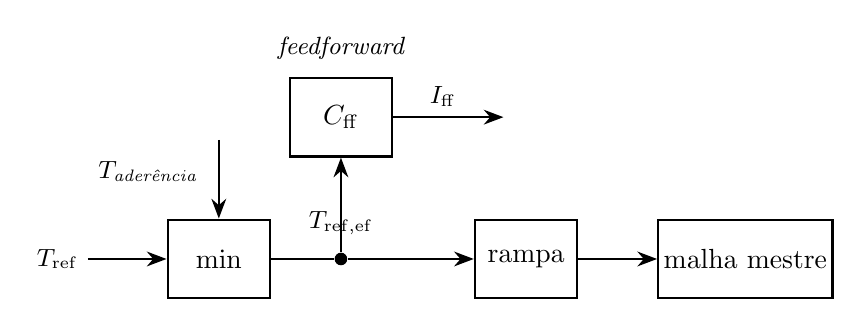
\begin{tikzpicture}[
  block/.style={draw=black, thick, minimum height=10mm, minimum width=13mm, inner sep=2pt},
  sign/.style={font=\itshape\small},
  arr/.style={-{Stealth[length=2.5mm]}, thick},
  arr open/.style={-Stealth[length=2.5mm], thick},
  node distance=8mm and 10mm,
]
\node[sign] (tref) {$T_{\mathrm{ref}}$};
\node[block, right=of tref] (min) {min};
\node[sign, anchor=east] at ($(min.north)+(-1.5mm,6mm)$) {$T_{\text{ader\^{e}ncia}}$};
\draw[arr] ($(min.north)+(0mm,10mm)$) -- (min.north);
% no de derivacao logo apos o min
\node[circle, fill=black, minimum size=1.6mm, inner sep=0pt, right=8mm of min] (dot) {};
\node[sign, above=1mm of dot] {$T_{\mathrm{ref,ef}}$};
% ramo que sobe para o feedforward
\node[block, above=12mm of dot] (cff) {$C_{\mathrm{ff}}$};
\node[sign, above=1mm of cff] {feedforward};
\draw[arr] (dot) -- (cff);
% saida do feedforward, seta aberta
\draw[arr] (cff.east) -- ++(14mm,0) node[sign, above, pos=0.45] {$I_{\mathrm{ff}}$};
% linha principal: rampa -> malha mestre
\node[block, right=16mm of dot] (rampa) {rampa};
\node[block, right=of rampa] (mestre) {malha mestre};

\draw[arr] (tref) -- (min);
\draw[thick] (min) -- (dot);
\draw[arr] (dot) -- (rampa);
\draw[arr] (rampa) -- (mestre);
\end{tikzpicture}%
}
\end{document}
